\documentclass{beamer}
\usepackage{fontspec}
\usepackage{polyglossia}
\usepackage{multicol}
\usepackage{luabidi}
\usepackage{xcolor}
\usepackage{graphicx}
\usepackage{float}
\usepackage{wrapfig}

\setmainlanguage{arabic}
\setotherlanguage{english}
\newfontfamily\arabicfont[Script=Arabic, Scale=1.0]{Amiri}
\setsansfont{Amiri} %(c) You have to put this extra command with {beamer} for the arabic language.
\newfontfamily\englishfont{Latin Modern Roman}
% \setmainlanguage[numerals=western]{arabic} %(c) For using Arabic numbers instead of the Indian.
\newcommand{\ar}{\textarabic}
\newcommand{\en}{\textenglish}


% \usetheme{Warsaw}
% \usetheme[progressbar=frametitle]{metropolis} %(c) that didn't work with the arabic so I used this:
\usetheme{metropolis}
% \setbeamertemplate{frame numbering}[fraction]%(c) is not good with the arabic.
\useoutertheme{metropolis}
\useinnertheme{metropolis}
\usefonttheme{metropolis}
\usecolortheme{spruce}
\setbeamercolor{background canvas}{bg=white}

\definecolor{ferngreen}{rgb}{0.31, 0.47, 0.26} %(c) I defined this color for the theme
\usecolortheme[named=ferngreen]{structure}
\definecolor{mytextgreen}{rgb}{0.0, 0.65, 0.31} %(c) I defined this color for the text below 

% \setbeamercovered{transparent=15} %(c) It applies only on \onslide command.

\title{محاكاة شبكة المثال 3-2 من كتاب التحليل على برنامج \en{ETAP} و نمذجة حساب قوانين مؤشرات المفاقيد للخطوط والعقد على برنامج \en{MATLAB}}
\author{إعداد الطالب : محمد علي قطان \en{207047}}
\institute{
  مقرر: تحليل نظم القدرة الكهربائية\\[2pt]
  إشراف: د. خالد شيخ حمود\\[2pt]
  }
\date{\small التاريخ : \en{31} كانون الثاني/يناير \en{2026}}

\setbeamertemplate{headline}{
  \begin{beamercolorbox}[wd=\paperwidth,ht=2.2cm,dp=0.8cm]{}
  \begin{picture}(0,0)
  \put(270,-25){
\includegraphics[width=2.3cm]{logo.png}}
  \end{picture}
  \begin{picture}(0,0)
    \put(30,20){%
        \parbox[t]{5cm}{% %(c) this command determines the width of the content (without triping). 
        \raggedright
        \normalsize %(c) Some commands change the size of there content; this command prevents the size change form being applied.
        \fontsize{8pt}{11pt}\selectfont 
        \hspace{21pt}\textbf{جامعة حلب}\\
        \hspace{-11pt}كلية الهندسة الكهربائية والإلكترونية\\
        قسم نظم القدرة الكهربائية
        }
      }
    \end{picture}
  \end{beamercolorbox}
}


\begin{document}
%(c) In Beamer we create frames to hold all of our information, a frame can contain a single slide in your slide presentation, or it can actually contians multiple slides 

  \begin{frame}
    \vspace{-1.4cm}
    \titlepage
  \end{frame}

\setbeamertemplate{headline}{} %(c) To remove the header from the next slides.

  \begin{frame}{المقدمة}
    تهدف هذه الدراسة إلى تحليل ظروف عمل شبكة قدرة كهربائية معطاة، وحساب مؤشرات المفاقيد النوعية للخطوط والعقد، والتي تُستخدم لتقييم أداء الشبكة وتحديد الأجزاء الأكثر تأثيرًا على المفاقيد.

في هذا العمل، تم أولًا نمذجة الشبكة الكهربائية المدروسة وتشغيلها باستخدام برنامج \textbf{\en{ETAP}}، وذلك للحصول على قيم الجهود عند العقد وقيم الاستطاعة الفعلية والردية المتدفقة في الخطوط. بعد ذلك، تم استخدام برنامج \textbf{\en{MATLAB}} لتطبيق القوانين الرياضية الخاصة بحساب مؤشرات المفاقيد النوعية، حيث تم حساب مؤشري المفاقيد الفعلية ($\lambda'$) والمفاقيد الردية ($\lambda''$) لكل خط ولكل عقدة في الشبكة.

تهدف النتائج المستخلصة من هذه المؤشرات إلى تقييم ظروف التشغيل الحالية للشبكة، وتمهيدًا لاستخدامها في تحسين تشغيل الشبكة وتقليل المفاقيد قدر الإمكان.

  \end{frame}

  \begin{frame}{وصف الشبكة المدروسة}
    تتألف الشبكة الكهربائية المدروسة من مجموعة من العقد المترابطة بواسطة خطوط نقل، حيث تُعطى قيم الاستطاعة الفعلية والردية للأحمال عند العقد، بالإضافة إلى قيم الجهود الاسمية لكل عقدة. كما تتوفر قيم الاستطاعة الفعلية والردية في بداية ونهاية كل خط، مما يسمح بحساب مفاقيد الاستطاعة على الخطوط.

    تم اعتماد هذه المعطيات كأساس لتحليل ظروف عمل الشبكة، وحساب مؤشرات المفاقيد النوعية، وذلك بالاعتماد على نتائج سريان الاستطاعة.\\

    \begin{columns}
      \begin{column}{0.6\textwidth}
        \textbf{التحقق من تماثل الشبكة:}
          يتم البدء بملاحظة أن الشبكة غير متماثلة كهربائياً؛ لأن نسبة المفاعلة إلى المقاومة ($X/R$) ليست ثابتة لكل أجزاء الشبكة (كما يظهر في الجدول 3-1)، وهذا يعني أن شرط التماثل الكهربائي (الشرط 3-8) غير محقق.\\
      \end{column}
      \begin{column}{0.4\textwidth}
        \centering
        
\includegraphics[width=1\textwidth]{Ph1.png}
      \end{column}
    \end{columns}

  \end{frame}

  \begin{frame}{محاكاة الشبكة باستخدام برنامج \en{ETAP}}
    تمت نمذجة الشبكة الكهربائية المدروسة باستخدام برنامج \textbf{\en{ETAP}}، حيث تم تمثيل العقد وخطوط النقل وفق المعطيات المعطاة في المثال، مع تحديد مستويات الجهد الاسمية وقيم الأحمال عند كل عقدة.

    \begin{figure}[H]
      \centering
      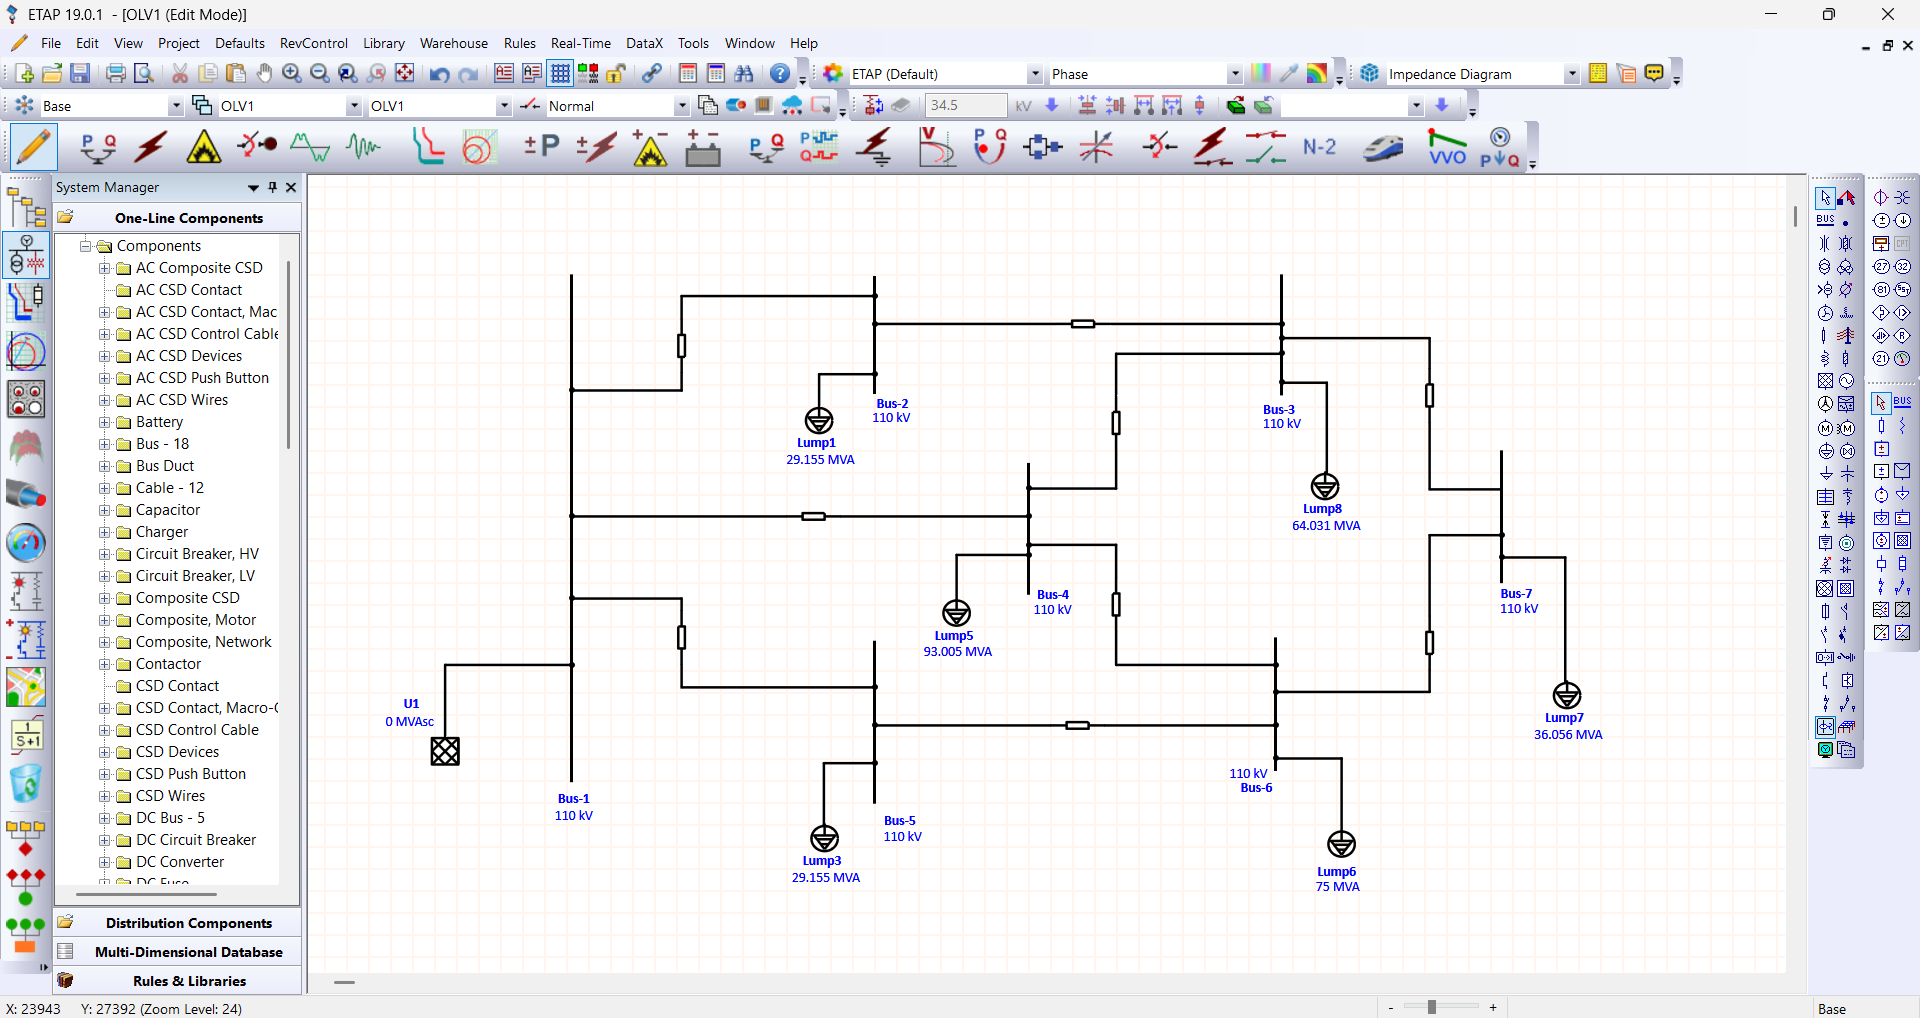
\includegraphics[width=0.8\textwidth]{etap_before.png}
      \caption{الشبكة على برنامج \en{ETAP}}
      \label{fig:etap_before}
    \end{figure}

  \end{frame}
  \begin{frame}{محاكاة الشبكة باستخدام برنامج \en{ETAP}}
    يوضح الشكل السابق مخطط الشبكة بعد نمذجتها وقبل تشغيل سريان الحمولة، حيث تظهر جميع مكونات الشبكة دون إظهار القيم التشغيلية.

    بعد ذلك، تم تشغيل دراسة سريان الحمولة (\en{Load Flow Analysis}) باستخدام برنامج \en{ETAP}، بهدف الحصول على الجهود عند العقد وقيم الاستطاعة الفعلية والردية المتدفقة في الخطوط.
  \end{frame}
  \begin{frame}{محاكاة الشبكة باستخدام برنامج \en{ETAP}}
    \begin{figure}[H]
      \centering
      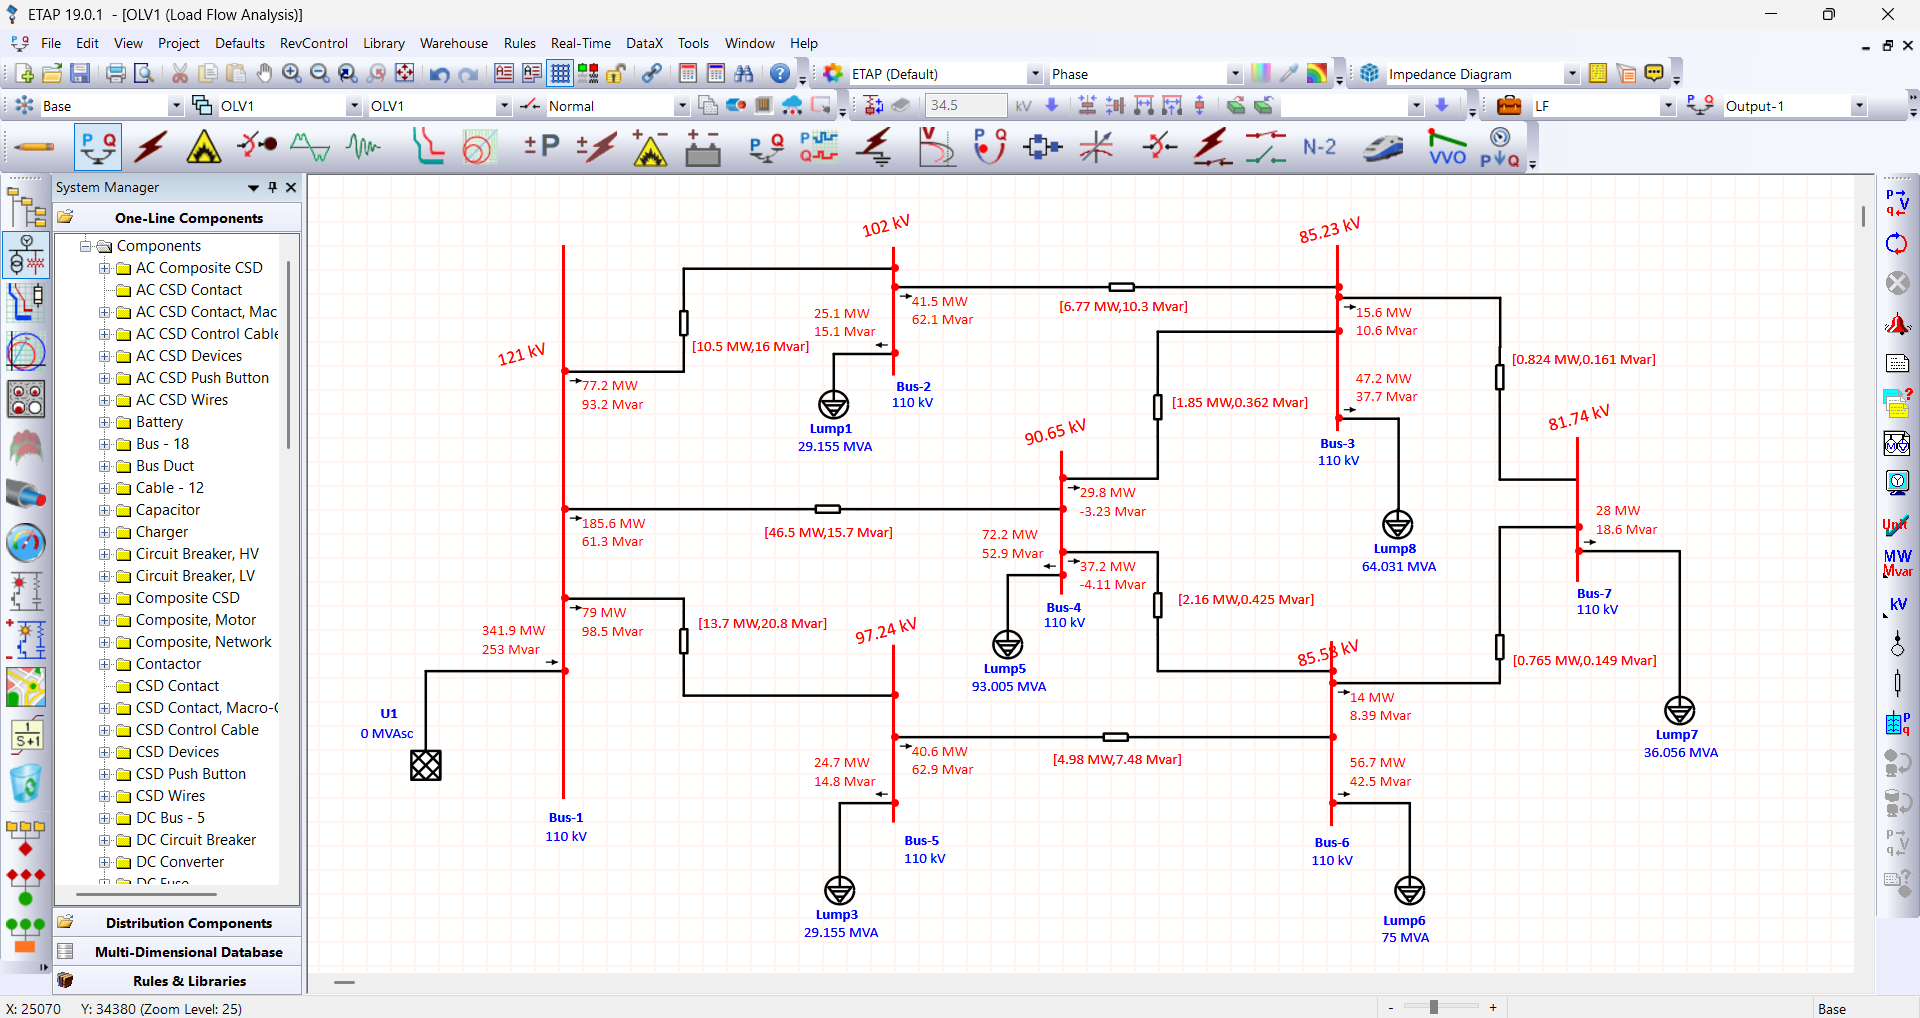
\includegraphics[width=0.9\textwidth]{etap_after.png}
      \caption{الشبكة بعد تشغيلها}
      \label{fig:etap_after}
    \end{figure}
    \vspace{-10pt}
    تبين الصورة السابقة نتائج تشغيل الشبكة، والتي تم اعتمادها لاحقًا في حساب مؤشرات المفاقيد النوعية باستخدام برنامج \en{MATLAB}.
  \end{frame}

  \begin{frame}{حساب مؤشرات المفاقيد باستخدام \en{MATLAB}}
    بعد الحصول على نتائج سريان الحمولة من برنامج \en{ETAP}، تم استخدام برنامج \textbf{\en{MATLAB}} لتطبيق القوانين الرياضية الخاصة بحساب مؤشرات المفاقيد النوعية للخطوط والعقد في الشبكة المدروسة.
    
    تم اعتماد قيم الاستطاعة الفعلية والردية في نهاية الخطوط، والتي تم الحصول عليها بطرح مفاقيد الاستطاعة من القيم في بداية الخط، بالإضافة إلى قيم الجهد عند نهاية كل خط ومقاومات الخطوط. وبالاعتماد على هذه القيم، تم حساب مؤشري المفاقيد الفعلية ($\lambda'$) والمفاقيد الردية ($\lambda''$) لكل خط وفق العلاقات التالية:
    \vspace{10pt}
    \begin{columns}
      \begin{column}{0.5\textwidth}
        \begin{equation}
          \lambda' = \frac{2 P_{\text{end}} R}{U^2}
        \end{equation}
      \end{column}
      \begin{column}{0.5\textwidth}
        \begin{equation}
          \lambda'' = \frac{2 Q_{\text{end}} R}{U^2}
        \end{equation}        
      \end{column}
    \end{columns}
    حيث تمثل $P_{\text{end}}$ و $Q_{\text{end}}$ الاستطاعة الفعلية والردية في نهاية الخط بعد طرح المفاقيد، ويمثل $R$ مقاومة الخط، ويمثل $U$ الجهد عند نهاية الخط.
    
  \end{frame}
  \begin{frame}{حساب مؤشرات المفاقيد باستخدام \en{MATLAB}}
    \begin{figure}
      \centering
      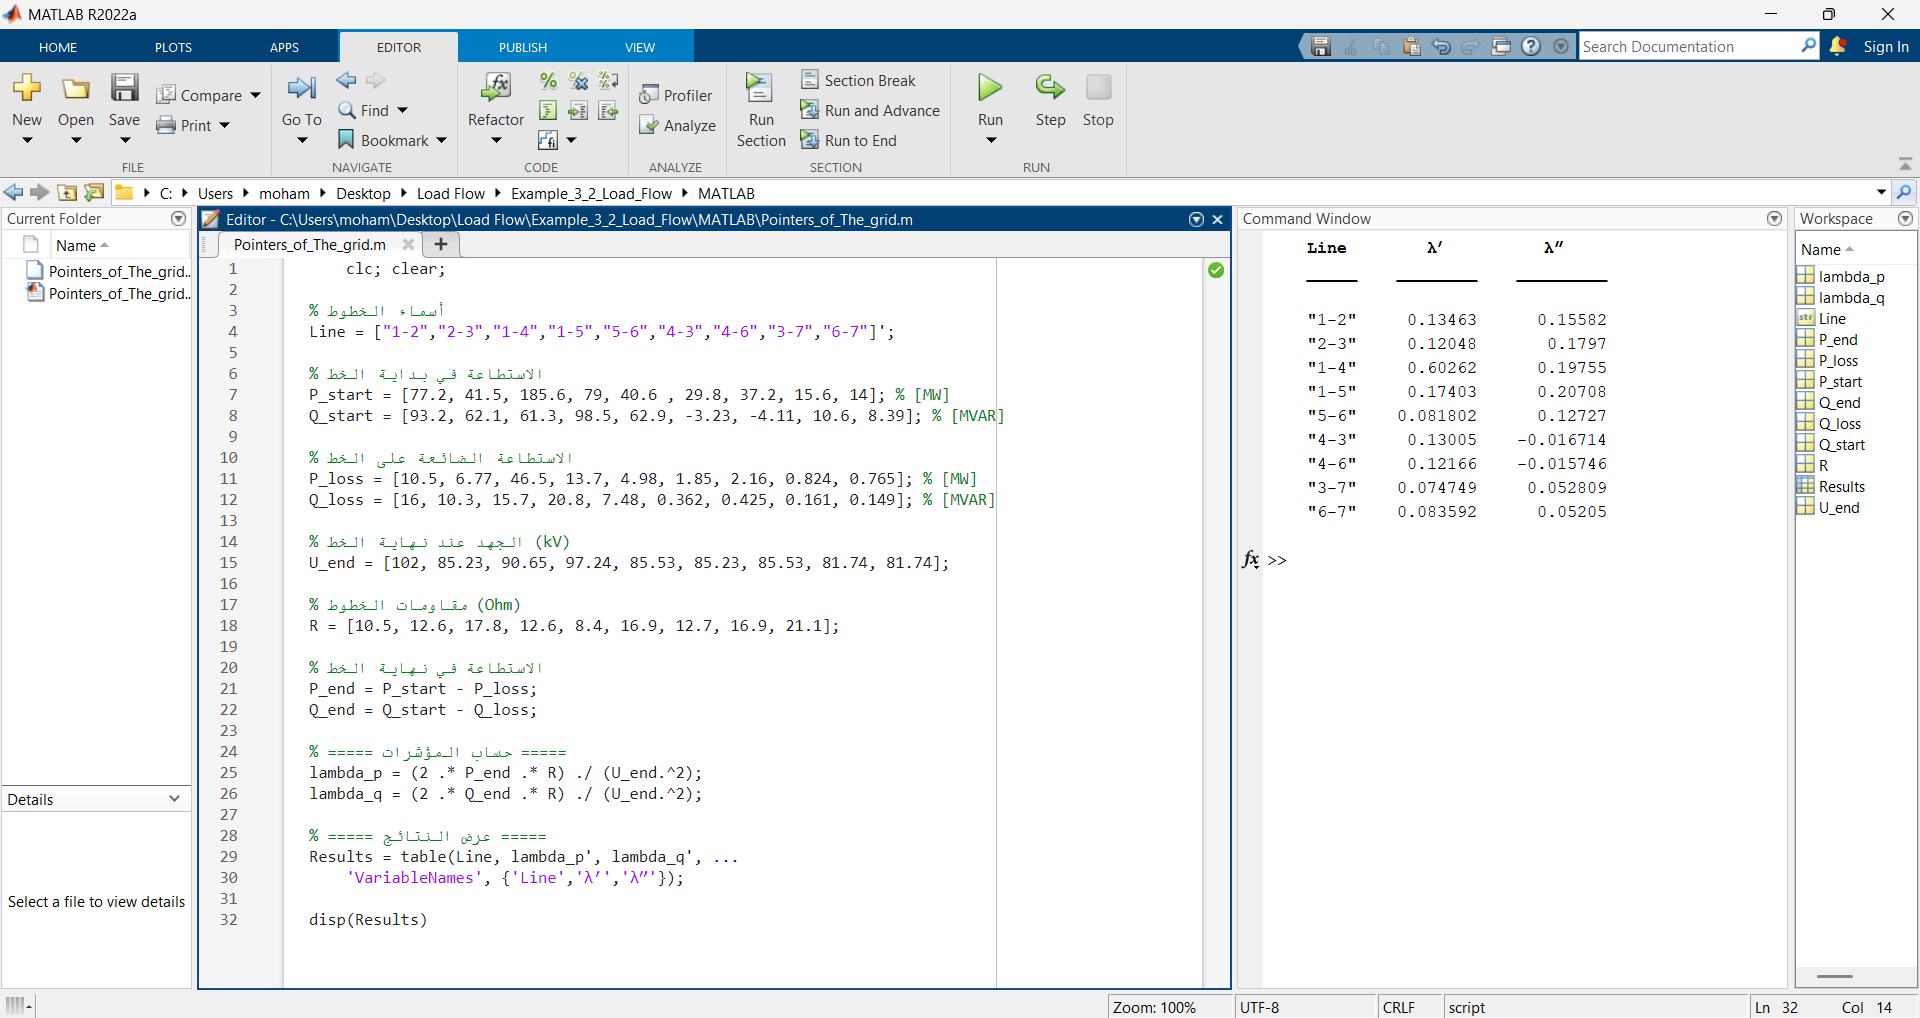
\includegraphics[width=1\textwidth]{matlab_2.png}
    \end{figure}
    الصورة السابقة توضح ادخال قيم الاستطاعة الفعلية والردية في بداية الخط والجهد في نهاية كل خط وكذلك ضياعات الاستطاعة على الخط حيث تم بعدها حساب الاستطاعة في نهاية الخط ثم تنظيم جدول في مؤشرات مفاقيد الاستطاعة الفعلية والردية.
  \end{frame}

  \begin{frame}{حساب مؤشرات المفاقيد باستخدام \en{MATLAB}}
\textbf{حساب مؤشرات المفاقيد عند العقد:}\\
نظرًا لأن مؤشرات المفاقيد تُحسب أساسًا على مستوى الخطوط، فقد تم حساب مؤشرات المفاقيد عند العقد من خلال تجميع قيم مؤشرات الخطوط الواقعة على المسار الواصل من العقدة المرجعية إلى العقدة المدروسة. ولتحقيق ذلك، تم تعريف المسارات التي تربط العقدة المرجعية ببقية العقد في الشبكة، بحيث يمثّل كل مسار مجموعة من الخطوط المتتالية.

\vspace{10pt}
\begin{columns}
  \begin{column}{0.60\textwidth}
    في برنامج \en{MATLAB}، تم تمثيل كل مسار على شكل مجموعة من فهارس الخطوط، حيث تشير هذه الفهارس إلى مواقع الخطوط المقابلة لها في مصفوفات مؤشرات المفاقيد. بعد ذلك، تم حساب مؤشرات المفاقيد الفعلية والردية لكل عقدة عن طريق جمع قيم مؤشرات الخطوط المكوّنة للمسار الخاص بها.
  \end{column}
  \hspace{-25pt}
  \begin{column}{0.4\textwidth}
    \centering
    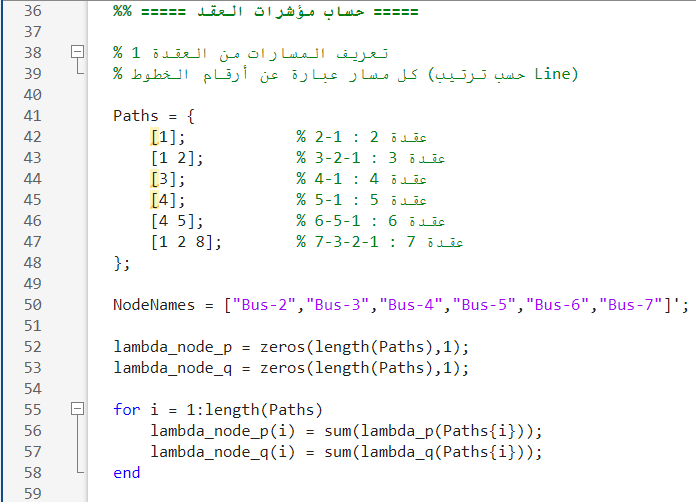
\includegraphics[width=1.1\textwidth]{matlab_3.png}
  \end{column}
\end{columns}

  \end{frame}

  \begin{frame}{حساب مؤشرات المفاقيد باستخدام \en{MATLAB}}
    \textbf{معالجة نقاط التفرع في الشبكة:}\\
    في بعض العقد، قد تتوفر أكثر من مسار كهربائي يصل العقدة المرجعية بالعقدة المدروسة، وذلك نتيجة iوجود نقاط تفرع في الشبكة. وبسبب عدم التماثل الكهربائي بين هذه المسارات، قد تختلف قيم مؤشرات المفاقيد المحسوبة لكل مسار.\\

    \vspace{10pt}
    \begin{columns}
      \begin{column}{0.45\textwidth}
        لذلك، تم حساب مؤشرات المفاقيد لكل مسار على حدة، ومن ثم اعتماد القيمة الوسطية لهذه المؤشرات لتمثيل المؤشر النهائي للعقدة المدروسة. وقد تم تطبيق هذه المنهجية، على سبيل المثال، عند العقدة (3) التي يمكن الوصول إليها عبر مسارين مختلفين، حيث تم أخذ المتوسط الحسابي لقيم مؤشرات المفاقيد الناتجة عن هذين المسارين.
      \end{column}
      \hspace{-30pt}
      \begin{column}{0.55\textwidth}
        \centering
        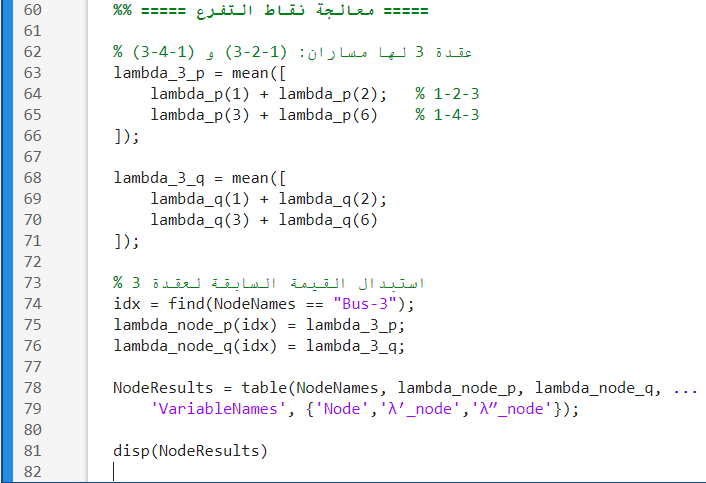
\includegraphics[width=1.1\textwidth]{matlab_4.png}
      \end{column}
    \end{columns}
  \end{frame}

  \begin{frame}{حساب مؤشرات المفاقيد باستخدام \en{MATLAB}}
سمحت هذه الآلية بحساب مؤشرات المفاقيد عند العقد بشكل منظم، مع مراعاة تأثير بنية الشبكة وتعدد المسارات، مما يوفّر تمثيلًا أدقّ لتوزع المفاقيد في الشبكة المدروسة.

\begin{figure}[H]
  \centering 
  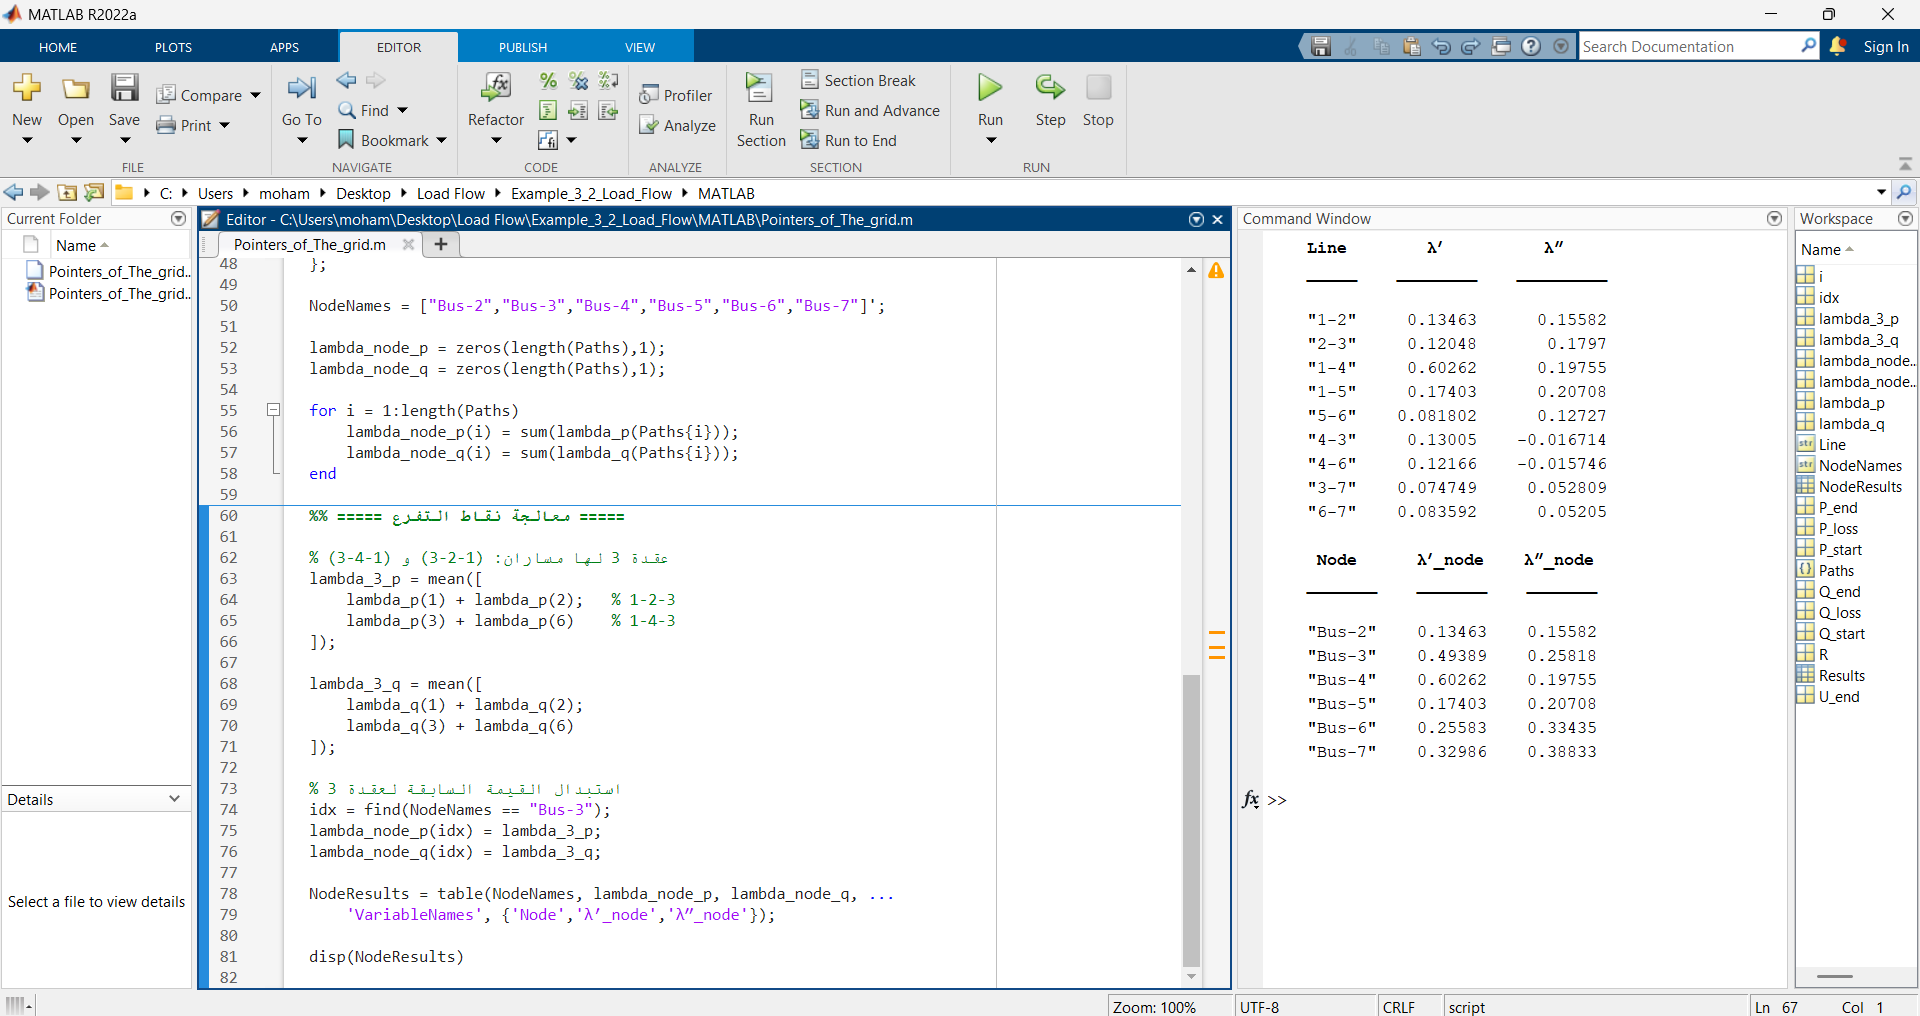
\includegraphics[width=1\textwidth]{matlab_5.png}
\end{figure}
  \end{frame}

  \begin{frame}{حساب مؤشرات المفاقيد باستخدام \en{MATLAB}}
    \begin{columns}
      \begin{column}{0.5\textwidth}
        \textbf{عرض النتائج:}\\[5pt]
        يبين الجدولان التاليان قيم مؤشرات مفاقيد الاستطاعة الفعلية ($\lambda'$) والردية ($\lambda''$) المحسوبة لكل من خطوط الشبكة والعقد، وذلك بالاعتماد على نتائج سريان الحمولة والقوانين الرياضية المعتمدة. توفّر هذه المؤشرات تصورًا كميًا لتوزع المفاقيد ضمن الشبكة، كما تُستخدم لتحديد الخطوط والعقد الأكثر تأثيرًا على المفاقيد، الأمر الذي يمهّد لاستخدامها في تحسين ظروف التشغيل وتقليل المفاقيد.
      \end{column}
      \hspace{-10pt}
      \begin{column}{0.5\textwidth}
        \centering
        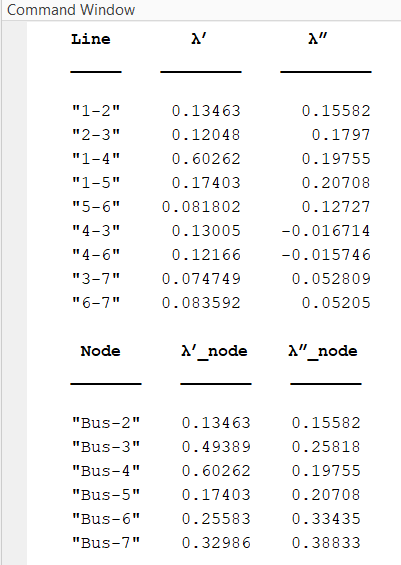
\includegraphics[width=0.95\textwidth]{matlab_6.png}
      \end{column}
    \end{columns}

  \end{frame}

  \begin{frame}{اتخاذ القرار الهندسي والنتائج النهائية}
    تشير المراجع إلى وجود عدة طرق هندسية للتغلب على عدم التماثل الكهربائي في الشبكات، مثل فتح الشبكات الحلقية، تعديل ممانعات الخطوط، واستخدام تجهيزات تنظيم سيالات الاستطاعة. في هذا العمل، تم التركيز على الحلول البرمجية من خلال تحليل مؤشرات المفاقيد النوعية باستخدام الحاسوب، لما تتميز به من بساطة وقلة كلفة وإمكانية المقارنة بين عدة سيناريوهات تشغيلية.

وقد تم اختبار خيار فتح الشبكة الحلقية عند عدة نقاط مرشحة، إلا أن نتائج المحاكاة أظهرت أن التشغيل الحلقي يحقق أقل مفاقيد قدرة فعلية للشبكة المدروسة، مما يدل على أن الحلول الأخرى المذكورة، رغم فعاليتها النظرية، تقع خارج نطاق هذا العمل.

  \end{frame}



\end{document}